%%%%%%%%%%%%%%%%%%%%%%%%%%%%%%%%%%%%%%%%%%%%%%%%%%%%%%%%%%%%%%%%%%%%%%%%%%%%%%%%%%%%%
% Template revision history:
% BS02022: Revised by Sukumar Natarajan, s.natarajan@bath.ac.uk
% BS2021: Revised by Filip Jorissen, filip.jorissen@kuleuven.be
% BS2019: Revised by Alessandro Prada, alessandro.prada@unitn.it
% BS2017: Initial version by Michael Wetter, mwetter@lbl.gov
%%%%%%%%%%%%%%%%%%%%%%%%%%%%%%%%%%%%%%%%%%%%%%%%%%%%%%%%%%%%%%%%%%%%%%%%%%%%%%%%%%%%%

\documentclass[twocolumn, a4paper,10pt]{article}
\usepackage[top=2.5cm, bottom=2.5cm, left=2.0cm, right=2.0cm,
columnsep=0.8cm]{geometry}
\usepackage{enumitem}
\usepackage[hidelinks]{hyperref}
\usepackage{boxedminipage}
\usepackage{nopageno}
\usepackage{graphicx}
\usepackage{natbib}
\usepackage[font=it]{caption}
\usepackage[usenames,dvipsnames]{xcolor}
\usepackage{listings}
\usepackage{caption}
\usepackage{subcaption}
%-----------------------------SET SKIP SPACES -------------------------------------------------------------------
\setlength{\abovecaptionskip}{0pt}
\setlength{\belowcaptionskip}{3pt}
\setlength{\parindent}{0pt}
\setlength{\parskip}{3pt}
%\renewcommand{\baselinestretch}{0.7}
% FOR enumerates
\setlist{itemsep=-0.1cm,topsep=0.1cm,labelsep=0.3cm}
\setenumerate{leftmargin=*}
\setcounter{secnumdepth}{-1}
%-----------------------------SET FONTS -------------------------------------------------------------------
% Set fonts for title, section and subsection headings
\makeatletter
\renewcommand\title[1]{\gdef\@title{\fontsize{12pt}{2pt}\bfseries{#1}}}
\makeatletter
\renewcommand\section{\@startsection{section}{1}{\z@}{3pt}{3pt}{\normalfont\large\bfseries}}
% \normalfont\large
\makeatletter
\renewcommand\subsection{\@startsection{subsection}{1}{\z@}{\z@}{\z@}{\normalfont\normalsize\bfseries}}
\makeatletter
\renewcommand\subsection{\@startsection{subsection}{1}{\z@}{\z@}{0.1pt}{\normalfont\normalsize\bfseries}}
\renewcommand\refname{References}
%END OF THE SETUP
%%%%%%%%%%%%%%%%%%%%%%%%%%%%%%%%%%%%%%%%%%%%%%%%%%%%%%%%%%%%

%%%%%%%%%%%%%%%%%%%%%%%%   TITLE   %%%%%%%%%%%%%%%%%%%%%%%%%%%%%%%
%%% Please keep the \vspace{4pt} at the top
\title{%
Executive summary for: Lethal Autonomous 
Weapon Systems\\																								% Line 1
%%% Please keep the \vspace{4pt} between lines in the title
\vspace{4pt}
Real world cases and Humanitarian implications \[LM-32 a.a. 2023/2024\]
} 																																% Line 2 
%If there is no second line then just put \phantom{Line 2} here
%%% Change or delete text before "\\" on the lines below to keep the layout but don't remove the "\\"
%%% Do not exceed more than 6 lines for authors and affiliations
\author{																																														% Line 3
Emmanuele Virginio Coppola$^1$, Mattias Trettel$^2$, Andrea Ceron$^2$\\ 																										% Line 4
$^1$ emmanuele.coppola@studenti.unitn.it\\ 																																	% Line 5
$^2$mattias.trettel@studenti.unitn.it\\
$^2$andrea.ceron@studenti.unitn.it\\
% comment the lines below and add \phantom{} lines as needed to reach a total of 10 lines
%\textit{(The names and affiliations SHOULD NOT be included in the draft submitted for review)}\\ 			 			  	% Line 7
%\textit{(leave blank up to line 10 - remove line numbering from final version)}\\ 															% Line 8
\phantom{Line 9}} 																																									% Line 9
\date{\vspace{-0.5cm}}	% remove default date and replace the Blank 10th line														% Line 10
%END OF THE TITLE
%%%%%%%%%%%%%%%%%%%%%%%%%%%%%%%%%%%%%%%%%%%%%%%%%%%%%%%%%%%%
\begin{document}

\maketitle
\begin{figure}
  \centering


\includegraphics[scale=0.6]{img/Logo.pdf} 																																	% Line 6 																																	% Line 6																																														% Line 3
\end{figure}
\section*{Introduction}	% Section headings need to be upper and lower case.
\addtocounter{section}{1}
Nowadays, artificial intelligence is a much-debated topic, and as of now, there isn't a proper regulation governing the use of AI. Despite numerous attempts to establish a set of laws and restrictions to clarify what is permissible and what isn't in this field, one thing always eludes every attempt at limitation: military use of AI. Although it might seem counterintuitive, given that the military domain is the most sensitive of all, it is also the most unrestricted regarding what can be done with AI. But is that really the case? In reality, there are principles that every military should adhere to the so-called International Humanitarian Laws. Unfortunately, while not legally binding, these principles constitute a guideline for proper conduct, always within limits, as the line between right and wrong, as we'll see, isn't as clear-cut as one might wish it to be. There are numerous instances where entire military operations have been halted because they were particularly complex from this ethical standpoint in a constant battle between those who wish to intervene and those who want to abort the operation. This is the way humans act, or at least, ideally. But what would happen if a machine were in our place? If there's one thing computers are not yet able to replicate, it's consciousness. So, how can we program them in a way that ensures they behave correctly? Given that here, a "mistake" could result in deaths and destruction. And even if it were possible to instill consciousness in a machine, whose consciousness would it be? The programmer's, the general's, or someone else's? Unfortunately, in this case, there is no answer, or rather, it's so complicated that it doesn't exist in its entirety. What we can do is try to set limits on what objectively seems wrong, this is precisely what the four principles aim to do, although every situation is subject to different interpretations.
\section*{The 4 Humanitarian principles}
\begin{itemize}
\item \textbf{The infliction of unnecessary suffering:} \\ This principle underscores the importance of minimizing harm and avoiding unnecessary suffering. In ethical discussions, particularly in the context of armed conflict, it suggests that any actions taken should be proportionate and justifiable, with the goal of minimizing the overall suffering inflicted on individuals.
\item \textbf{The principle of proportionality:} \\ This principle dictates that the use of force should be proportional to the threat or harm faced. In the context of armed conflict, for example, it implies that the level of force used in response to an attack should be proportionate to the severity of the threat. The goal is to prevent excessive or disproportionate use of force that could lead to unnecessary harm.
\item \textbf{The notion of necessity:}\\Necessity in this context refers to the idea that any action or use of force should be necessary to achieve a legitimate goal. It emphasizes that force should only be employed when there are no reasonable alternatives and when it is essential for achieving a just and lawful objective. This principle is closely linked to the idea of minimizing harm and ensuring that actions are justified.
\item \textbf{The principle of humanity:}\\The principle of humanity emphasizes the importance of treating individuals with dignity and compassion, particularly in times of conflict or crisis. It underscores the need to safeguard the well-being of all individuals, regardless of their affiliation. This principle is often associated with international humanitarian law and human rights, guiding actions to ensure a basic level of humanity even in challenging circumstances.
\end{itemize}

What will happen when these principles are not applied by machines? And if those machine are the ones with feelings and emotions? Like humans?
\section*{Yugoslav Wars}
We have already seen in the recent history of mankind what happens when we have a war where no principle is applied.
Often described as one of Europe's deadliest armed conflicts since World War II, the Yugoslav Wars were marked by many war crimes, including genocide, crimes against humanity, ethnic cleansing, and mass wartime rape. 

\section*{Drone kills its operator}

\begin{itemize}
\item \textbf{Abstract}
\item \textbf{Key innovations}
\item \textbf{Practical implications}
\item \textbf{Introduction}
\item Methods
\item Results
\item Discussion
\item \textbf{Conclusion}
\item Acknowledgments
\item Nomenclature
\item \textbf{References}
\end{itemize}
Optional parts can be replaced according to the needs but the order should be preserved.\\
Second level paragraphs are acceptable. Lower level paragraphs are discouraged.\\
Do not leave empty lines between titles, paragraphs and figures in the main body. Use paragraph spacing above and below titles and paragraphs as specified in the following. \\
In case you use MS-Word, you can refer to the predefined styles in the gallery included in the MS-word template (in alphabetical order):
\begin{itemize}
\item Authors
\item Captions
\item Equation
\item Figure
\item List (bulleted)
\item List (numbered)
\item Heading 1
\item Heading 2
\item Normal
\item Reference
\item Tables
\item Title
\end{itemize}
%---------------------------------------------------------------------------------------
\section*{Parts of the paper: top section}
%---------------------------------------------------------------------------------------
The top section of the first page of the paper is used for the title of the paper, list of authors, and authors' affiliation. This section always consists of 10 lines of exactly 14 points spacing, in single column format.
\subsection*{Title, authors, and authors' affiliations}
Titles (MS-word: select \textit{Title style}) should be in bold font size 12 points. Do not use more than 2 lines for the title, and try to limit it to ten words.\\
Authors (MS-word: select \textit{Authors style}), authors' affiliations, and other information should be in font size 12 points. In case of more than one affiliation, reference superscripts after the author's names and before the corresponding affiliation will be added.\\
Authors' affiliations (MS-word: \textit{always in Authors style}), can include contact (e-mails, telephone numbers, postal address, etc.) and other information. However, the 10 lines limitation applies. If you need less than 10 lines for all the information, please leave the remaining lines blank.
%---------------------------------------------------------------------------------------
\section*{Main body}
%---------------------------------------------------------------------------------------
After the 10 lines in the top section, the rest of the document is in two-column format, with a space between the two columns of 80 mm. The space between the columns should be centred on the paper. Line spacing is exactly 12 points.\\
The main text should be typed in 10 point font, justified, with 3 points spacing below each paragraph (\textit{MS-word: select \textit{Normal style}}).\\
The headings of each section should use font size of 12 point, capitalized, with 3 and 3 points spacing above and below (\textit{MS-word: select \textit{Heading 1 style}}). The headings of the subsection should use 10 points size and bold, with 3 points spacing below (\textit{MS-word: select \textit{Heading 2 style}}). Left alignment is used for headings. Both the sections and subsections \underline{\textbf{should not}} be numbered.
%---------------------------------------------------------------------------------------
\subsection*{Abstract}
%---------------------------------------------------------------------------------------
The abstract of your paper should be about 100 words.\\
Abstracts must clearly identify (i) what is the current state of the art, (ii) what are its deficiencies, (iii) what methods have been applied, (iv) what are the results, and (v) what is the lasting contribution of the submission.
%---------------------------------------------------------------------------------------
\subsection*{Key inovations}
%---------------------------------------------------------------------------------------
In 1-5 bullet points, clearly highlight where this paper moves beyond the state of the art.
%---------------------------------------------------------------------------------------
\subsection*{Practical implications}
%---------------------------------------------------------------------------------------
The practical implications section should be about 20 - 50 words.\\
Capture succinctly what a simulation practitioner should take away from your paper: always do \ldots ; avoid  \ldots; consider x and beware of y in case of  \ldots

%---------------------------------------------------------------------------------------
\subsection*{Figures and Tables}
%---------------------------------------------------------------------------------------
Figures and Tables are preferably included in the text where they are discussed rather than at the end of the paper. In the case of figures, select the ``In line with text" from the layout options if you use MS-Word. A centred alignment with 3 and 3 points spacing above and below is required (\textit{MS-word: select \textit{Figure style}}). \\
Both figures and tables must have a number and caption. Figure~\ref{fig:fig01} (\textit{refer this way to a figure in the text, do not use Fig. ~\ref{fig:fig01} or figure ~\ref{fig:fig01}}) is an example of a graph in the text. Captions (\textit{MS-word: use \textit{Captions style}}) always follow the figure in italic font size 10 points, and centred, with 3 and 3 points spacing above and below.\\
If figures authorship does not belong to one of the authors, authors are required to ask to the copyright owner the permission to use that material and to provide a proof that the permission has been accorded.\\
Colour images are welcome.\\
\begin{figure}
\centering
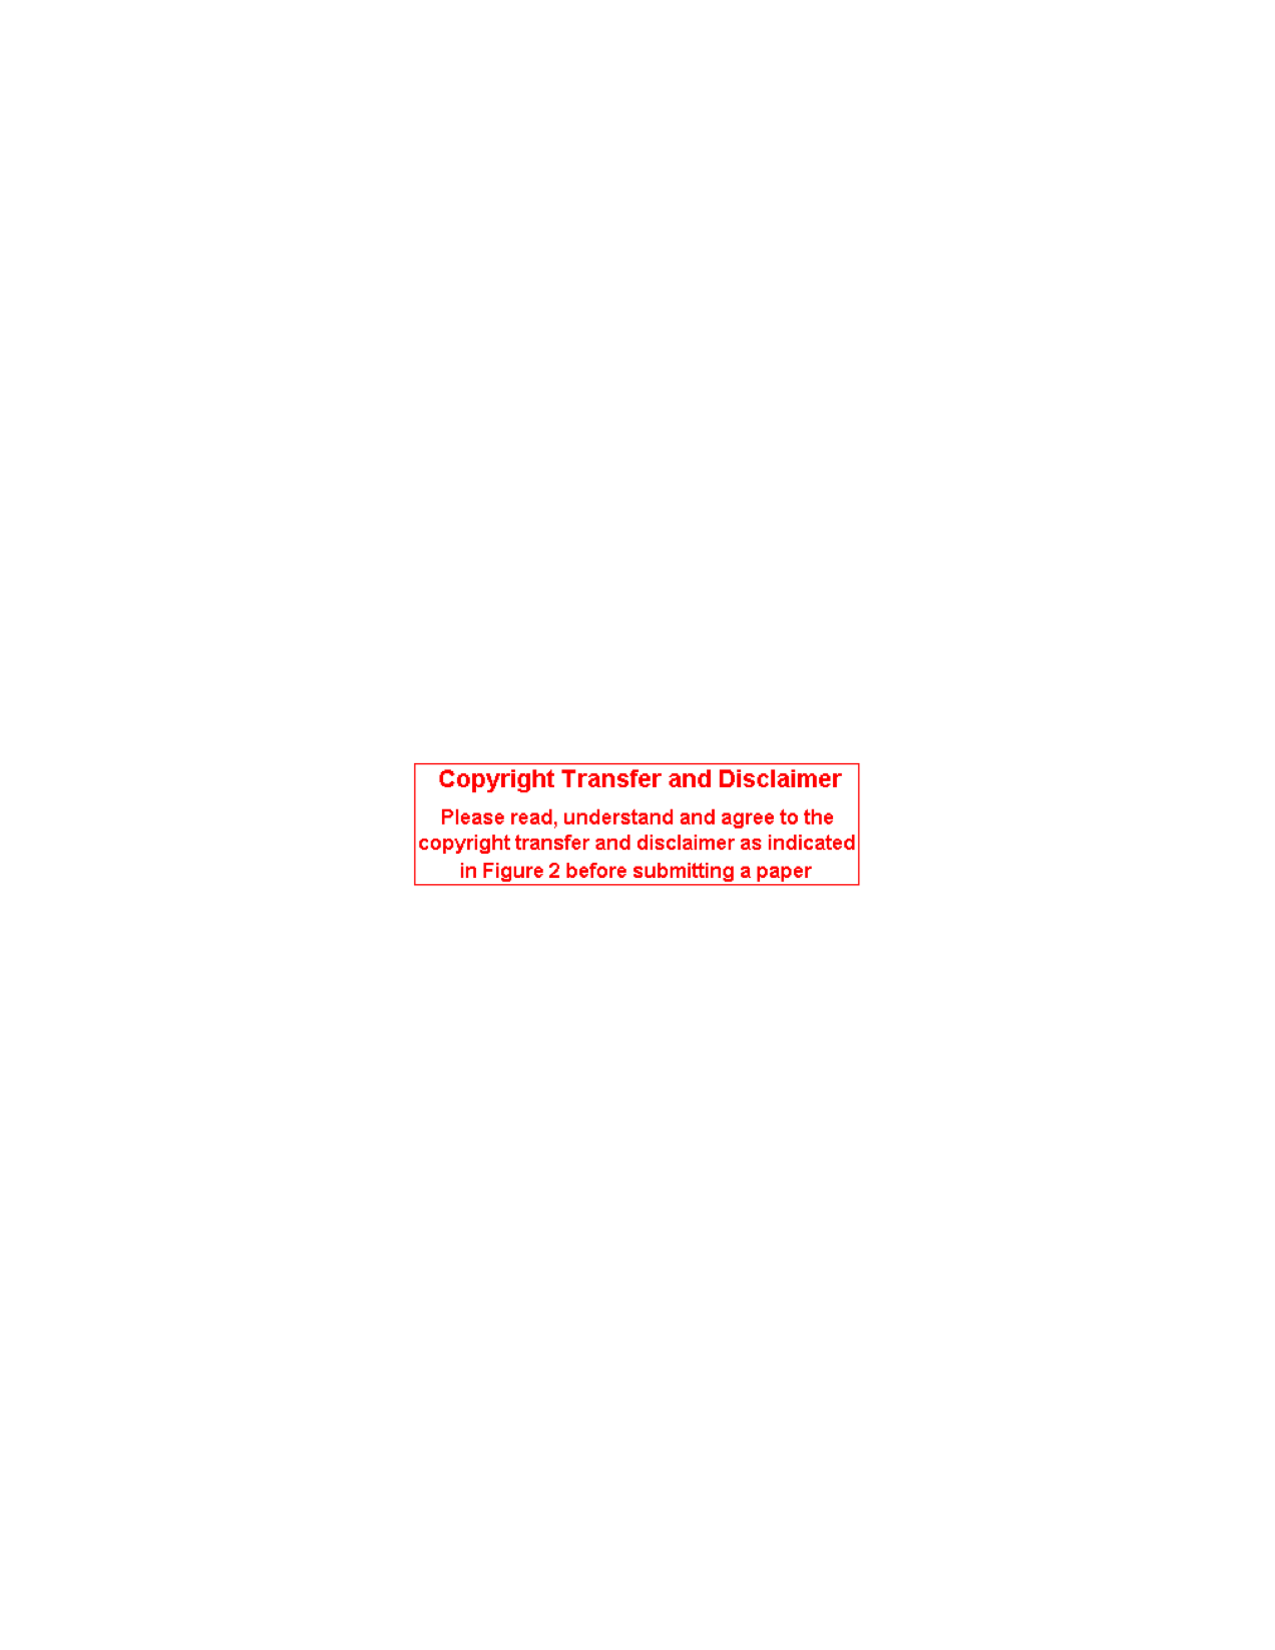
\includegraphics[scale=1.0]{img/fig1.pdf}
\caption{A gentle reminder.}
\label{fig:fig01}
\vspace{-16pt}   % Please use appropriate negative vspace to remove the space above/belovw the Table
\end{figure}
Table \ref{tab:tab01} shows an example of a table, where the caption should be on the top of the table, with the same format as figure captions. Text in tables can be in font size of 9 points and centred, with no spacing above and below (MS-word: use \textit{Tables style}).
\begin{table}[ht]
\vspace{-5pt}   % Please use appropriate negative vspace to remove the space above/belovw the Table
\caption{Example of a table.}
\label{tab:tab01}
\centering
\begin{tabular}{| c | c | c | }
  \hline
  \bf{Heading 1} & \bf{Heading} 2 & \bf{Heading 3} \\
  \hline
  Entry 1 & Entry 2 & Entry 3 \\
  \hline
\end{tabular}
\vspace{-5pt}   % Please use appropriate negative vspace to remove the space above/belovw the Table
\end{table}
Oversized figures and tables may be included in the text. However, authors may arrange the layout properly so that it appears at the top or the bottom of the page, or preferably on a separate page at the end of the paper. Figure ~\ref{fig:fig02} is an example of an oversized figure.
%---------------------------------------------------------------------------------------
\subsection*{Equations and units}
%---------------------------------------------------------------------------------------
Each significant equation or formula should be displayed on a separate line. Center equations and place consecutive equation numbers flush right in parentheses. For example,
\begin{equation}\label{eq:example}
  a^2+b^2=c^2.
\end{equation}
If you use MS-Word, use the Equation style and use tabs to position equations and equation numbers correctly.
Mathematical symbols should be clear and avoid ambiguities. Keep using font size 10 points. Symbols representing physical quantities (or variables) are italic. Symbols representing units, operators, labels and numbers, are regular (upright).\\
Equations should be referenced in the text by their number (\ref{eq:example}). A brief description of the symbols used in your paper should be added in a nomenclature section at the end of the text or inline with the text where the symbols are first used.\\
SI units of measurement are mandatory. If other units are mentioned, always provide their equivalent value according to SI.\\
SI notation must be adopted as regards symbols, prefixes and other writing rules. In particular comma as a decimal separator is preferred to the point (which is anyhow allowed if used consistently throughout the manuscript). If needed, only blank spaces are allowed as thousand separators.
%---------------------------------------------------------------------------------------
\subsection*{References}
%---------------------------------------------------------------------------------------
All publications cited in the text should be listed at the end of the Main body in a References section, in alphabetical order of the family name of the first author. From the second line on, each entry should be indented by 5 mm. Justified alignment with 3 and 3 points spacing above and below each paragraph must be used (\textit{MS-word: select \textit{Reference style}}). Examples of reference style are reported in the reference section below for journals, conference proceedings, books and technical standards.\\
In the main text, refer to a reference using author-year style such as \citet{Clarke2015:1} or \citet{ChuMajumdar2012}. When the reference is not a part of the sentence, use the author-year style in brackets (\cite{Clarke2015:1, ChuMajumdar2012,Monarim2014, BSDO2011, Mahdavi2011,iso52017}).
%---------------------------------------------------------------------------------------
\subsection*{Bulleted and numbered lists}
%---------------------------------------------------------------------------------------
Numbered and bulleted lists must be justified, with no indentation, and 5 mm hanging. You may use List (bulleted) or List (Numbered) styles in MS-Word.
%---------------------------------------------------------------------------------------
\section*{If you use MS-Word}
%---------------------------------------------------------------------------------------
You can use the .docx document as a template if you use MS-Word. Please use the style for each section as has been defined in the template. You can either use the template, rename it, and cut-and-paste your paper from other document(s) into the template, or you can use your document, open style organizer (Format – Style and then click ``organizer"), delete all your styles and import the styles from the template.
If you use the template, do not forget to disable the line number on the Top section of the first page before you submit the paper and cancel instructions comments (\textit{in brackets and italic fonts}).
%---------------------------------------------------------------------------------------
\section*{If you use \LaTeX}
%---------------------------------------------------------------------------------------
Please use the \LaTeX template you can download from the conference website. In the compressed folder, you will find:
\begin{itemize}
\item \textbf{format guide.tex}: a fill-in form for a standard article with usage comments. Please copy it to a new file with a new name and use it as the basis for your article.
\item \textbf{reference.bib}: is a plain text containing the database of the references used for the format guide. Please use the same entries included in this file for your database.
\item \textbf{BSO2022.bst}: this is the bibliography style of the BS2021 conference proceedings, which we are using for BSO 2022. 
\end{itemize}
%---------------------------------------------------------------------------------------
\section*{Submission instruction}
%---------------------------------------------------------------------------------------
\begin{enumerate}
    \item To enable the blind review process please do not include your name and affiliation on the draft submitted for review. This information will be requested in the final submission.
    \item Please convert your entire document to PDF format. An additional doc/\LaTeX version of the manuscript can be optionally added. In this case a single .zip file including both the .pdf and the doc/\LaTeX files of your contribution shall be uploaded.
    \item Papers must be at most 8 pages long.
    \item You can use any file name, but please do not use special characters, umlaute, etc.
    \item The maximum file size is 10 MB, but please use vector graphics where possible to reduce your file size.
		\item If your paper has not met all the requirements for submission, your file \textbf{will not be processed for review and you will be requested to resubmit}. If everything is in order, the paper will be up-loaded to the review area of the conference web site.
\end{enumerate}
%---------------------------------------------------------------------------------------
\section*{Conclusion}
%---------------------------------------------------------------------------------------
This paper has shown how to prepare a paper for submission to Building Simulation and Optimisation Conference 2022. Good luck with your paper. 
%---------------------------------------------------------------------------------------
\section*{Acknowledgment}
%---------------------------------------------------------------------------------------
This document is a summary of various documents from previous Building Simulation Conferences.
%here starts the references
\bibliographystyle{BSO2022}
\bibliography{references}
\newpage
\onecolumn
Please \textbf{do not} include this disclaimer in your paper.  You will be required to accept these conditions when you  submit your paper via the web site.

\begin{figure*}[ht]
\centering
\begin{boxedminipage}{\textwidth}
Building Simulation 2021
 
I or we, the author(s) and presenter(s) of the conference contribution ``Automatic generation of second level space boundary geometry from IFC models'', have read the following Copyright Transfer and Disclaimer, and agree to them by submitting the final contribution materials.
 
 \begin{enumerate}
 \item The author(s) and presenter(s) will automatically grant to IBPSA-England a nonexclusive, royalty-free, perpetual, worldwide, irrevocable, sub-licensable, and transferable license to publish the abstract(s), research paper(s) and/or presentation(s) and/or digital posters (with unmodified content) in any fashion (including but not limited to inclusion in the Building Simulation and Optimisation 2022 printed and electronic proceedings, via electronic means such as the world wide web, and inclusion in future compilations of presentations, also including online-exploitation via electronic means in order to organize an e-conference, regardless of the accessibility through paying registration). This ``nonexclusive'' license means that the author(s) are not restricted as to future use of the material except that exclusive rights cannot be granted to another.
 
\item The author(s) and presenter(s) grant and assign to IBPSA-England or its agent the nonexclusive rights to record the presentation at the BSO 2022. These rights give IBPSA-England the unlimited license to use, modify (format, not content), sell and distribute the recorded presentation (including voice of the presenter(s)).
 
\item The author(s) and presenter(s) affirm that they have the right to grant the license specified in (1) and (2), that is, publication by IBPSA-England or its licensees will not be in conflict with existing copyright or other restrictions.
 
\item The author(s) and presenter(s) acknowledge that acceptance of the abstract(s), research paper(s) and/or presentation(s) does not imply IBPSA-England's endorsement of or agreement with the ideas presented. It is understood that IBPSA-England does not accept responsibility for any content within the abstract(s), research paper(s) and/or presentation(s) that may be found to be libelous, infringing on copyright or other intellectual property rights, invading individual privacy or to be otherwise unlawful. Under no circumstances shall IBPSA-England be liable for any damages resulting from use of information included in the presentation.
 
\item Finally, the undersigned confirms that he/she has the power and authority to make and execute this agreement. For jointly authored works the signing author/presenter signs as authorized agent for the others.
 \end{enumerate}


\end{boxedminipage}
\caption{The author will be required to accept these conditions when they submit their paper via the web site.}
\label{fig:fig02}
\end{figure*}

\end{document}
